\documentclass[plainsections,32pt]{sciposter}

\usepackage[brazil]{babel}		% Idioma do documento
\usepackage{xcolor}			    % Controle das cores
\usepackage[T1]{fontenc}		% Selecao de codigos de fonte.
\usepackage{graphicx}			% Inclusão de gráficos
\usepackage[utf8]{inputenc}		% Codificacao do documento (conversão automática dos acentos)
\usepackage{wallpaper}
\usepackage{wrapfig}
\usepackage{amsfonts,amssymb,amsmath,amsthm}
\usepackage{multicol}
\usepackage{anyfontsize}
\usepackage{braket}
\usepackage{anyfontsize}

\providecommand{\U}[1]{\protect\rule{.1in}{.1in}}
%EndMSIPreambleData
\setcounter{tocdepth}{4}

%opening
\definecolor{amarelo}{HTML}{FFCC00}
\definecolor{verde}{HTML}{006600}
\renewcommand{\papertype}{custom}
\setlength{\paperwidth}{90cm}
\setlength{\paperheight}{100cm}
\renewcommand{\setpspagesize}{
\ifthenelse{\equal{\orientation}{portrait}}{
\special{papersize=90cm,100cm}
}{\special{papersize=90cm,100cm}}}
\setlength{\topmargin}{0in}
\setlength{\headheight}{0in}
\setlength{\headsep}{0in}
\setlength{\textheight}{84cm}
\setlength{\textwidth}{75.5cm}
\setlength{\oddsidemargin}{2.4cm}
\setlength{\evensidemargin}{0cm}
\setlength{\parindent}{0.25in}
\setlength{\parskip}{0.25in}
\setlength{\pdfpagewidth}{90cm}
\setlength{\pdfpageheight}{100cm}
\newcommand\BackgroundPic{
\put(-82,65){
\parbox[b][\paperheight]{\paperwidth}{
\vfill
\centering

\includegraphics[width=\paperwidth,height=\paperheight,
keepaspectratio]{poster-xi-sic.jpg}
\vfill
}}}
\setlength{\columnseprule}{0pt}

\renewcommand{\titlesize}{\fontsize{84}{45}\selectfont }
\newcommand{\largo}{\fontsize{36}{40}\selectfont }
\makeatletter



% Redefine a função section
\renewcommand\section{\@startsection {section}{1}{\z@}{-1ex \@plus -0.5ex \@minus -.1ex}{0.8ex \@plus.1ex}{\largo\bfseries\fontsize{28}{26}\selectfont}}

\makeatother
\vspace{-1cm}

\def\thesection{}
%%% Título %%%
\title{\vspace{-4cm} \hspace{-28cm}\textcolor{amarelo}{\parbox{0.9\textwidth}{Mapeamento Clássico-Quântico: \\ Um Estudo do Modelo de Ising em Duas Dimensões}}}
%%%
\usepackage{parskip}
\begin{document}

\AddToShipoutPicture{\BackgroundPic}
\makeatletter
\AddToShipoutPicture{%
            \setlength{\@tempdimb}{.5\paperwidth}%
            \setlength{\@tempdimc}{.5\paperheight}%
            \setlength{\unitlength}{1pt}%
            \put(\strip@pt\@tempdimb,\strip@pt\@tempdimc){%
                    }%
}
\makeatother
\maketitle
\mbox{}\vspace{0cm}

\begin{center}
\textbf{\textit{\large Alex Enrique Crispim}}\\
Centro de Ciências Naturais e Humanas - UFABC\\
Av. dos Estados, 5001, Santo André, SP\\
\textit{alex.enrique@ufabc.edu.br}
\end{center}

\vspace{1.5cm}
\begin{multicols}{2}
\paragraph{Resumo:} Neste trabalho, estudou-se a técnica do \textit{mapeamento clássico-quântico}, aplicado ao Modelo de Ising. O objetivo final do projeto era extrair informações da versão quântica do modelo unidimensão usando este formalismo. Isso se deu calculando computacionalmente observávais quântico, utilizando o modelo clássico bidimensional.

\textbf{Palavras-chave:} Modelo de Ising, Mecânica Quântica, Mecânica Estatística, Transição Quântica de Fase, Sistemas Quânticos de Muitos Corpos. Sistemas Fortemente Correlacionados.

\section*{Introdução}
O Modelo de Ising surgiu na década de 1920 como um modelo clássico simplificado para se estudar sistemas ferromagnéticos. Este modelo foi o primeiro a apresentar uma transição de fase, fato mostrado pela solução exata encontrada por L. Onsager (Onsager, 1944).

De forma geral, acredita-se que a função de partição de um modelo quântico de dimensão $D$ pode ser mapeada exatamente na função de partição de um modelo clássico de dimensão $D+1$. Este mapeamento tem sido fundamental para o estudo de teorias fortemente correlacionadas. Em especial, a aplicação deste formalismo ao Modelo de Ising leva à formulação de um modelo quântico de fundamental importância para o estudo de transições quânticas de fase e o entendimento de transições de fase de segunda ordem.

\section*{O Modelo de Ising} O Modelo Clássico de Ising em duas dimensões corresponde a uma rede de variáveis clássicas $\sigma_i$ que assumem valores $\pm 1$. Essas se encontram arranjados em uma rede bidimensional, normalmente quadrada e tem Hamiltoniana
\begin{equation}
  H_{cl.} = -J \sum_{\braket{i, j}} \sigma_i \sigma_j,
\end{equation}
com $\braket{i, j}$ representando os $j$ primeiros vizinhos de $i$.

A função de partição desta Hamiltoniana clássica, pode ser mapeada exatamente na função de partição da Hamiltoniana
\begin{equation}
  \hat{H}_{\Delta} = -J\sum_i \sigma_{i}^z \sigma_{i+1}^z + \Delta \sigma_i^x
\end{equation}
chamada \textit{Hamiltoniana Quântica de Ising Unidimensional}, com $\sigma^x$ e $\sigma^z$ representandos as matrizes $x$ e $z$ de Pauli.

A solução de Onsager mostra que o modelo clássico apresenta uma transição de fase à temperatura $T_c$ dada por
\begin{equation}
  \beta_c J = \frac{\log(1 + \sqrt{2})}{2}
  , \quad \beta_c = \frac{1}{kT_c},
\end{equation}
onde $k$ é a constante de Boltzman. Para o modelo quântico, a transição de fase se manifesta como $\Delta = 1$.

Utilizando a técnica do mapeamento clássico-quântico, é possível estudar o modelo quântico de Ising na transição de fase, por meio do modelo clássico. As vantagens se dão em termos de menor complexidade computacional e no uso de uma teoria clássica (mecânica estatística clássica), costumeiramente mais simples de se trabalhar.

\section*{Desigualdades de Bell e Correlações Quânticas}
Na década de 60, John Bell Derivou uma desigualdade sobre o valor esperado de variáveis aleatórias, sob as hipóteses do paradoxo EPR (paradoxo de Einstein-Podolsky-Rosen) (Bell, 1964). De forma reformulada e mais geral, a desigualdade afirma que o valor esperado da quantidade $QS + RS + RT - QT$, onde $Q, R, S, T$ são variáveis aleatórias que assumem valores $\pm 1$, é tal que
\begin{equation}
  \braket{QS + RS + RT - QT} \leq 2.
\end{equation}
Esta desigualdade se funda nos argumentos de Einstein, Podolsky  e Rosen acerca de uma possível incompleteza da Mecânica Quântica (Einstein \textit{et al}, 1935). O interesse nesta desigualdade foi a verificação de que a mesma é incorreta; o mundo comporta-se conforme a Mecânica Quântica.

Em especial, para o estado
\begin{equation*}
  \ket{s} = \frac{\ket{\uparrow \downarrow} - \ket{\downarrow \uparrow}}{\sqrt{2}}
\end{equation*}
o valor esperado na forma de (4) para os observáveis
\begin{equation}
  Q = \sigma_1^z, \quad R = \sigma_1^x, \quad S =  \frac{-\sigma_2^z - \sigma_2^x}{\sqrt{2}}, \quad T =  \frac{\sigma_2^z - \sigma_2^x}{\sqrt{2}}
\end{equation}
é igual a $2\sqrt{2} > 2$.

Supondo que primeiros vizinhos da cadeia unidimensional quântica pudesse estar emaranhados no estado $\ket{s}$, uma simulação do valor esperado (4) para estes observáveis deveria, em algum momento, violar a desigualdade de Bell. Para tal, simulou-se uma rede de spins clássios com a Hamiltoniana (1), calculando os observáveis $\sigma_{i}^x$, $\sigma_{i}^z$, $\sigma_{i+1}^x$ e $\sigma_{i+1}^z$ por meio do mapeamento entre os sistemas. Com estes observáveis e os observáveis definidos em (5), pode-se fazer o estudo requerido da desigualdade (4), indicando a presença do estado $\ket{s}$.


\section*{Resultados}
\begin{figure}
  \center
  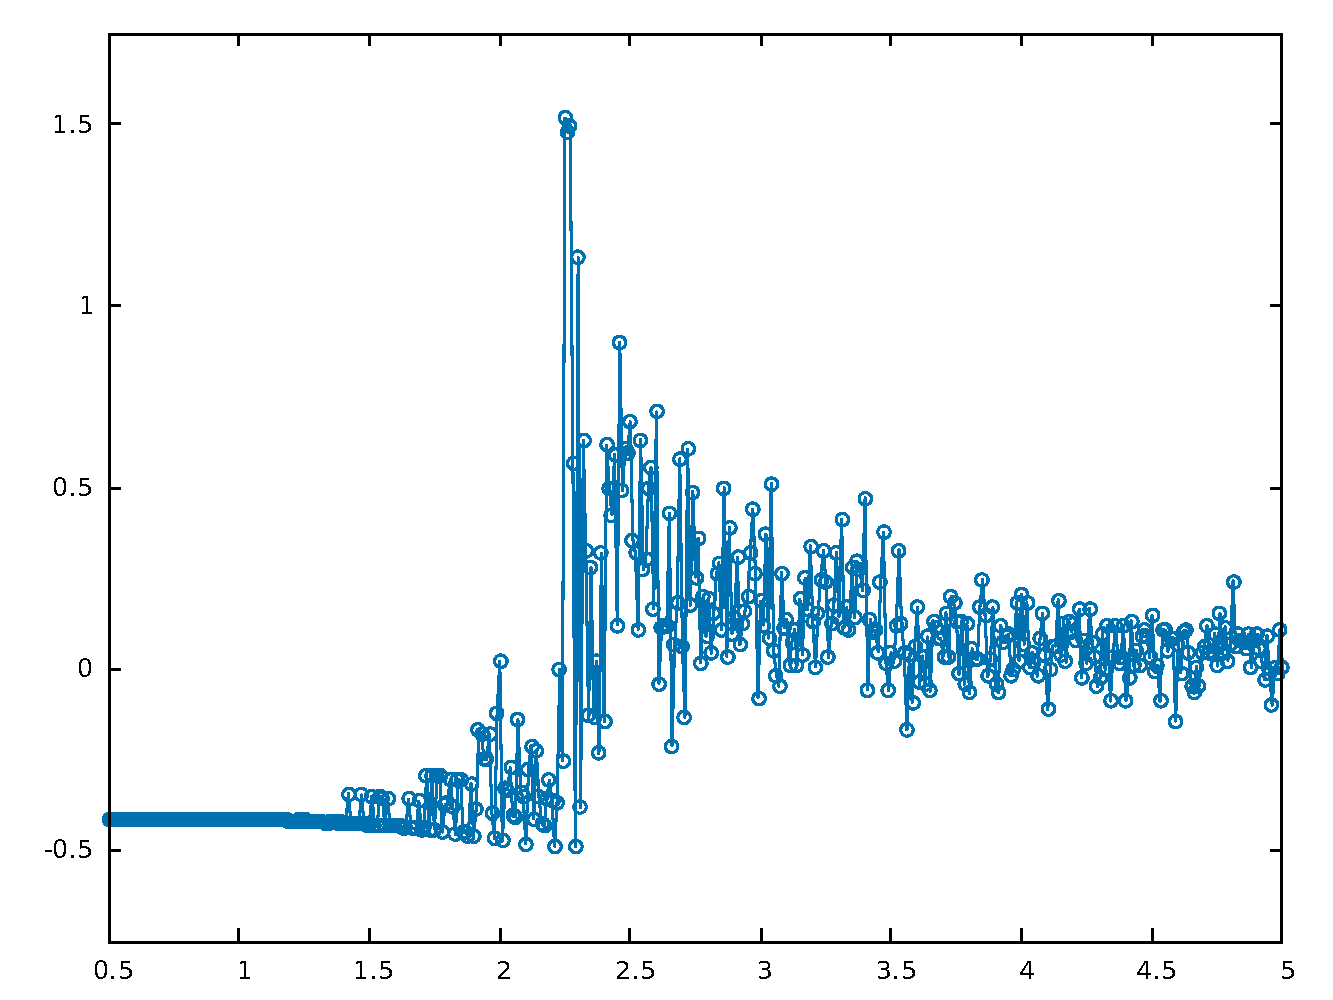
\includegraphics[scale = 1]{result3.pdf}
  \caption{}
\end{figure}




\section*{Conclusão}

\section*{Referências}

Onsager, L. (1944). ``Discussion'', Nuovo Cimento (suppl.) 6 , 261.

Bell, John. (1964). ``On the Einstein Podolsky Rosen Paradox''. Physics. 1 (3): 195–200.

Einstein, A.; Podolsky, B.; Rosen, N. (1935). ``Can Quantum-Mechanical Description of Physical Reality Be Considered Complete?''. Physical Review. 47 (10): 777–780

\section*{Agradecimentos}
Os alunos devem incluir em seus pôsteres uma seção de agradecimento com dizeres do tipo: Este trabalho foi financiado pelo Programa de Iniciação Científica da UFABC (PIC/UFABC) ou pelo CNPq (para bolsistas CNPq).


\clearpage % remover ao final

\end{multicols}

\end{document}
